\documentclass[ngerman]{article}

\usepackage[margin=2.75cm]{geometry}
\usepackage[T1]{fontenc}
\usepackage[utf8]{inputenc}
\usepackage{textcomp}
\usepackage{graphicx}
\usepackage{babel}
\usepackage{titlesec}
\usepackage{xcolor}



\begin{document}


\section*{Was ist Freifunk}
Bei Freifunk handelt es sich um ein Projekt zum Aufbau einer unabhängigen Netzinfrastruktur unter Nutzung der WLAN-Technik.

Dafür werden verwendet Standard-WLAN-Router verwendet, die aus dem privaten Hausgebrauch bekannt sein dürften. 
Auf einen solchen WLAN-Router wird eine speziellen Firmware (das Betriebssystem des WLAN-Routers) installiert, mittels der die Vernetzung von Freifunk-Geräten untereinander ermöglicht wird.
Die Freifunk-Firmware wird als Open Source Projekt dezentral in den regionalen Freifunk Verbänden entwickelt und interessierten zur freien Nutzung zur Verfügung gestellt.
Änderungen und Erweiterungen, die in einem regionalen Verband durchgeführt werden, stehen anschließend wiederum allen Verbänden zur freien Nutzung zur Verfügung.
   
Ein mit der Freifunk-Firmware ausgestatteter WLAN-Router ist in der Lage, weitere Freifunk-Geräte in seiner Nähe automatisch zu erkennen und sich mit diesen per WLAN zu verbinden. 
Es entsteht ein sogenanntes Mesh-Netzwerk, das sich dadurch auszeichnet, dass ein Knoten mit einer Vielzahl anderer Knoten verbunden ist.
Durch ein intelligentes Routing-Protokolls, das speziell für unzuverlässige Funknetze entworfen wurde, ist die Wegfindung innerhalb des Netzes und somit die Kommunikation untereinander möglich.

Die Abbildung zeigt, wie durch den Betrieb von Freifunk-Knoten in den Wohnungen von Bürgern ein miteinander verbundenes Netzwerk entsteht, das unabhängig von kommerziellen Anbietern funktioniert. Nutzer, die sich mit dem Freifunk-Netz verbinden können untereinander kommunizieren und Daten austauschen, ohne dass dazu ein Internetanschluss benötigt wird.


\begin{figure}[h!]
	\centering
	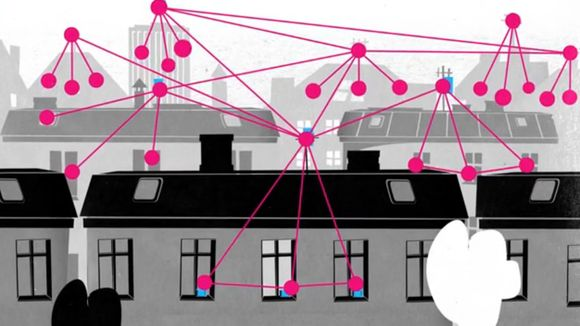
\includegraphics[width=.7\textwidth]{freifunk-mesh}
	%\caption{}
	\label{fig:freifunkwolke}
\end{figure}



\end{document}